\chapter{Introduction}\label{Intro}
Anyone who has had exposure to a second language (L2), even if for a brief amount of time, has likely noticed that the L2 may share some of the same words and lexical features with the first language (L1). For instance, in both Dutch and English the word \textit{hotel} refers to an establishment that provides lodging for guests. The word \textit{hotel} is a cognate in Dutch and English: a translation equivalent that shares similar lexical form in both languages (i.e., orthography and phonology). Words in two languages may also overlap in lexical form without sharing the same meaning; these are called false cognates or homographs. For example, the English translation of the Dutch word \textit{room} is cream. An example with more sinister consequences is the German word for poison: \textit{Gift}. While observations such as these may seem amusing when first learning a new language, it would seem absurd to assume that a proficient German-English bilingual would think of poison upon hearing the English word gift. However, this may not be far from the truth, as recent evidence suggests that bilinguals may not be able to function as the sum of two monolinguals \parencite[][]{Grosjean1989}.

While listening to spoken language, reading written text, or preparing words and sentences to be spoken, the bilingual appears to have both languages active momentarily before the intended language is selected \parencite[e.g.,][]{Dijkstra2005,Kroll2005,Marian2003}. Research initially suggested that the dominant L1 was more likely to intrude when bilinguals were performing a task in their weaker L2 \parencite[e.g.,][]{Dijkstra1999, Dijkstra1998}. More recent findings demonstrate that bilinguals' experience with an L2 or even L3 can also influence their performance when completing a task in the more dominant L1 \parencite[e.g.,][]{VanHell2002}. This parallel activation of the two languages has been referred to as \textit{language nonselectivity} and it manifests itself as a cross-language interaction when bilinguals encounter words that are ambiguous across the two languages (e.g., \textit{hotel} or \textit{room} when read by a bilingual who speaks Dutch and English). The observed interactions are not categorical but can be modulated by the relative degree of cross-language overlap \parencite[e.g.,][]{Schwartz2007}.

%The observation of parallel activation of two languages when only one is required has had profound consequences for our understanding of the bilingual experience. Critically, bilinguals are able to effectively juggle alternatives in both languages simultaneously without producing random errors of language in spontaneous speech (Poulisse, 1994). At the same time, it is a well-known fact that many bilinguals are able to code-switch with each other, changing languages effortlessly even within a sentence. These switches are often strategic in nature and follow a set of grammatical and social rules as opposed to being random slips of language (e.g., Myers-Scotton, 2002). The ability to negotiate parallel activation of the two languages, to exploit its presence during code-switching, and to avoid its consequences in single language discourse suggest that bilinguals develop the ability to exert control over language processes (e.g., Green, 1998). In fact, bilingualism appears to confer a set of measurable benefits in the realm of executive function (e.g., Bialystok, 2005). The hypothesis is that a life of learning to juggle the parallel activation of the multiple languages creates cognitive expertise that generalizes beyond language to attentional control. 
 
%As exciting as the cognitive consequences of language nonselectivity may be, 

Despite evidence for nonselectivity, under ordinary circumstances bilinguals must eventually select one language to read, hear, or speak. Most of the early studies that have found evidence for language nonselectivity were  conducted outside of any meaningful context; participants were required to make decisions about or name single words aloud. Without additional context, lexical ambiguity is at its peak. Thus, parallel activation may be a byproduct of the way in which word recognition experiments are performed rather than a feature of ordinary bilingual language processing. A set of recent studies has asked whether the evidence for language nonselectivity can also be observed within sentence context \parencite[][]{Baten2010,Chambers2009, Duyck2007, Libben2009, Schwartz2006, VanAssche2009, VanAssche2010, VanHell2008}. Using a range of experimental methods, these studies have converged upon the conclusion that sentence context in and of itself is not sufficient to constrain lexical access to one language. This is true when bilinguals listen to spoken words in the L2 \parencite[e.g.,][]{Chambers2009} or read the L2 \parencite[][]{Baten2010,Duyck2007, Libben2009, Schwartz2006, VanAssche2010, VanHell2008}. Parallel activation of the alternative language has also been observed when bilinguals read words in L1 sentence contexts \parencite[][]{VanAssche2009}. If sentence context itself cannot constrain language selection, then other factors must be doing so.

In typical language use, a sentence contains words grouped together in order to express a meaning. Two important and distinct aspects of this characterization are the meaning of the sentence (the semantics) and the rules that govern the ordering of words in the sentence (the syntax). Both the semantics and the syntax can impose restrictions or constraints on upcoming words in a sentence. For example, the sentence \textit{John kept his gym clothes in the locker} imposes a semantic restriction; the semantic context of the sentence (established by gym clothes) makes the word locker more predictable. This sentence is said to have a high semantic constraint. In such highly constrained contexts, monolingual readers experience facilitated processing of the  target word \textit{locker} \parencite[e.g.,][]{Schwanenflugel1988, Stanovich1983}. For bilinguals, semantic constraints may play a role in assisting with the selection of the intended language. When bilinguals read sentences with a high semantic constraint, they tend to access language-ambiguous words as if they were words in only the language of the sentence \parencite[e.g.,][]{Libben2009, Schwartz2006, VanHell2008}. That is, word recognition appears to be language-selective when ambiguous words appear in sentences that are semantically constrained.

%Similar to the example above, the sentence When the composer entered the hall, he sat at the bench and began to play the piano is highly semantically constrained. The context established by the meanings of the words composer, hall, and bench all converge on an interpretation of a music hall and therefore the word piano is predictable. Compare this to a sentence with a low semantic constraint: When we entered the dining hall we saw the piano in the corner of the room. Here the word piano could be nearly any other noun (e.g., cat, table, lamp). Critically in this example, the word piano is language ambiguous between English and Spanish; piano is a cognate. 

%When bilinguals read sentences with a low semantic constraint, they continue to activate both language interpretations of the cognate as if they were processing the word out of context. In contrast, when English-Spanish bilinguals read sentences that are highly constrained semantically, they appear to access the cognate as if it were a word only in the language of the sentence (e.g., Libben \& Titone, 2009; Schwartz \& Kroll, 2006; van Hell \& De Groot, 2008; but see van Assche, 2009).1 That is, word recognition appears to be language-selective when ambiguous words appear in sentences that are semantically constrained.

The majority of evidence supports the notion that semantics are completely or partially shared across the bilingual's languages \parencite[e.g.,][]{Costa1999, Fox1996, Kroll1992, Kroll1993, Potter1984, Schwanenflugel1986, Smith1991, Snodgrass1984}. Thus, there is no reason a priori that semantics itself should provide a solid language cue that would facilitate language selection. Furthermore, not every sentence is highly semantically constrained, so there must be other ways for bilinguals to arrive at the language of the sentence.

%How, then, could a highly biased context eliminate parallel activity of the unintended language? Recall the high constraint sentence When the composer entered the hall, he sat at the bench and began to play the piano. By the time the reader gets to the word piano, the set of lexical candidates has been heavily restricted and the potential candidates (e.g., musical instruments) have received activation. For a bilingual, this activation, in turn, may allow early selection of the intended language causing the reader to ignore the existence of piano in the unused language. However, the role of the semantics in curtailing parallel activity of the unintended language is indirect in nature and, hence, the effect may be reliable only under some circumstances. There must be other factors at work to enable bilinguals to select the intended language. After all, not all sentences are highly biased toward a specific meaning. What, in those cases, allows a bilingual to speak the target language?

%The past studies on reading language ambiguous words in context have examined the role of semantic constraints. However,

The semantics are not the only source of restrictions on upcoming words; the syntactic structure of the sentence also provides constraints. Importantly, the ways in which sentences achieve syntactic coherence differs markedly across languages (compared to semantics which are largely shared). In extreme cases, the word ordering of sentences differs across languages. To illustrate, whereas English uses a Subject-Verb-Object (e.g., \textit{The child sees the house}) word ordering, Fijian uses a Verb-Object-Subject ordering (e.g., \textit{Sees the house the child}). In these cases, the interpretation of the sentences does not differ between English and Fijian, but the syntax does. The case of Fijian and English is an extreme example, and more minor differences also occur across languages. For example, Spanish sentences can include special pronouns (called proclitics) and they  must drop the subject of an object relative clause. These two features are exemplified in \ref{lasmonjas} by \textit{le} and \textit{[pro]} respectively. 

\ex.\label{lasmonjas} Las monjas \textbf{le} llevaron las mantas que \textbf{[pro]} hab\'{i}an bordado a la directora del orfanato.\\
      The nuns \textbf{[ ]} took the quilts that \textbf{they} had embroidered to the director of the orphanage.

In contrast, English does not use proclitics nor does it allow for the dropping of the subject in a relative clause. These syntactic differences may provide salient cues to language and allow bilinguals to selectively access words in sentence context. 

The purpose of the current investigation is to further explore the mechanisms that allow bilinguals to control selection of the intended language by having participants read words either within or outside of a sentence context. In preparation for the upcoming experiments, I first review the bilingual word recognition literature, beginning with a sample of the out of context research and  the dominant word recognition model which explains the findings. Then I turn to a comprehensive review of the more recent in context research.

\section{Out of context word recognition}\label{Intro::OOC}
Evidence for nonselectivity is seen reliably when participants are asked to read, hear, or produce single words in one of the two languages. Many of these studies exploit the presence of ambiguities in the written form and pronunciation of words in the bilingual's two languages to demonstrate that bilinguals, but not monolinguals, are sensitive to the properties of the language not in use. Although evidence for nonselectivity has been found using a wide array of stimuli (e.g., cognates, homographs, and words with many cross-language neighbors), the \textit{cognate effect}, that cognates are typically recognized fast than noncognate controls, has been the most robust \parencite[e.g.,][]{Dijkstra1998}. Influence from the unintended language is seen regardless of whether the L2 or the L1 is in use \parencite[][]{Dijkstra1998, Grainger1992, Dijkstra1999, VanHell2002}. Furthermore, both phonological and orthographical representations remain active \parencite[e.g.,][]{Marian2003, Jared2001} regardless of script differences between the two languages \parencite[e.g.,][]{Gollan1997}

If a bilingual can selectively access one of her two languages, then words that are language-ambiguous should be recognized no differently than words that are language non-ambiguous. For this reason, language-ambiguous words have been the focus of many studies investigating lexical access in bilingual speakers. Two types of language-ambiguous words, cognates and homographs, are of particular interest to psycholinguists because they are the words that are the most ambiguous between languages. Sharing nearly complete overlap between two languages (similar orthography, phonology, and meaning), a cognate is the prime example of a language-ambiguous word. Homographs are also highly language-ambiguous, except that they do not share meaning. Therefore, it is reasonable to predict that cognates may allow for greater parallel activation of the two languages.

Dijkstra, Van Jaarsveld, and Ten Brinke  showed that cognates robustly allow for measurement of parallel activation of languages compared to homographs. In three separate experiments, they asked Dutch-English participants to make lexical decisions to single words. In the first two experiments, participants were told to make a ``yes'' decision for English, their L2. The  stimuli consisted of cognates, homographs, and English noncognate words. These stimuli were supplemented with a set of Dutch words in the second experiment. The Dutch words required a ``no'' response. In the third experiment, participants were told to respond ``yes'' to both Dutch and English words. In all three experiments, Dijkstra et al. found a facilitatory cognate effect. However, the nature of the homograph effect depended on the composition of the other stimuli and instructions of the task. 

%In experiment 1, which included no Dutch distractor words, homographs were not recognized differently from control words, but when Dutch words were included (experiment 2), an inhibitory homograph effect emerged.  The inclusion of Dutch words raised activation of Dutch, a language requiring a ``no'' response.  Thus participants had to be more cautious in their responses to words that seemed Dutch (including homographs). When participants were allowed to respond to either language in the third experiment, this caution was no longer necessary and participants could again rely on cross-language overlap especially at the level of orthography, causing homographs, like cognates, to become facilitated. Critically, there was always a cognate effect no matter the instructions or surrounding materials, suggesting that the cognate effect is relatively robust compared to the homograph effect. 

%\textcite{Dijkstra1998} provided evidence for the assumption that cognates may strongly activate both languages in bilingual speakers. In a series of experiments using the lexical decision task (LDT), Dijkstra et al. investigated the recognition of cognates and homographs by Dutch-English bilinguals. In a typical LDT, and the type that Dijkstra et al. use in two of their experiments, participants are asked to decide if target stimuli, displayed one at a time, are licit words in the language specified by the experimenter. Target stimuli consist of real words and nonword distractors. Nonword distractors, also called pseudo-words, follow the phonotactic properties of the language of the task. In an example of a typical LDT trial, a Dutch-English participant may have to decide if the word \textit{room} (a homograph) is a word in English (a so-called English lexical decision). Dijkstra et al. also employed what they call a \textit{general lexical decision task} in which participants respond \textit{yes} for a word that is in either of their two languages. In the first experiment, they included both cognates and noncognates in an English LDT. They found that participants were faster to recognize cognate words compared to non-ambiguous controls; this effect is commonly referred to as \textit{the cognate effect}. Furthermore, they found no difference in the recognition of homographs compared the controls. Two later experiments, in which they varied the task and materials, revealed a homograph effect. Importantly, the homograph effect emerged only after L1 words were included. For the purpose of the present study, two critical findings can be gleaned from Dijkstra et al. First, the cognate effect was witnessed regardless of the fact that there were no L1 words embedded in the stimuli. Conversely, the homograph effect needed to be given a boost in activation of the L1 in order to surface. The fact that a boost was necessary for the homographs to affect recognition is indicative that the homograph effect is weaker than the cognate effect. The second critical finding in this study is that L2 speakers of English are activating their L1 when they are participating in a task that is solely conducted in their L2. 

The evidence for parallel activation of the stronger L1 when using the weaker L2 may not be surprising. In fact, it seems obvious that a more dominant system would impede on a less dominant one. However, parallel activation is not simply a function of language dominance or proficiency. Tasks where bilinguals use only the more dominant L1 have yielded a striking and counterintuitive result: knowledge of a second language influences how bilinguals use their first language. \textcite{VanHell2002} asked highly proficient Dutch-English-French trilinguals to participate in a Dutch lexical decision task. The participants were recruited in the Dutch language and were given no knowledge that either French or English were in any way involved in the study. The LDT contained Dutch words in each of the following categories: cognates between Dutch and French but not English (e.g., Dutch: meuble [French: meuble; English: piece of furniture]), cognates between Dutch and English but not French (e.g., Dutch: bakker [English: baker; French: boulanger]), and noncognate controls (Dutch: fiets [French: vélo; English: bike]). The stimuli also contained a set of Dutch pseudo-words. Pseudo-words, like the nonwords above, follow the phonotactic regularities of a language but have no meaning (e.g., raponse in Dutch or wug in English). The results of the study showed that participants were reliably faster to judge Dutch-English and Dutch-French cognates as words than noncognate controls. The participants believed that this task was conducted only in Dutch and had no reason to suspect that English or French was in any way involved. Yet, they could not prevent the activation of their L2 and L3 when they are reading the cognate words. This result demonstrates that the bilingual language processing system functions in a nonselective manner even when recognizing words in the stronger L1.

Thus far, we have seen evidence for parallel activation when bilinguals process language-ambiguous words in either their L1 or L2. A question that now arises is how deep this parallel activation runs. In the two studies above, bilinguals were performing LDTs that involved reading words. Thus, we have learned that the orthography of both languages is active. Although cognates are said to overlap in both orthography and phonology, there can actually be subtle differences between them across languages. For example, while base, a cognate, is written identically in English and Spanish, the pronunciations are noticeably different. Thus it's reasonable to suspect that the phonology of the cognates plays a role in their recognition as well. 

\textcite{Schwartz2007} looked at the role of phonology in more detail. In this study, instead of the LDT, participants were asked complete a word naming task. Words appear one at a time on a computer screen and they are asked to name the word aloud; the reaction time (RT) to the onset of articulation is measured. The word naming task is similar to the LDT in that it measures recognition of the word; however, in addition, the naming task requires participants to select a single word and access its phonology. Schwartz and Kroll embedded Spanish cognates and their English translations into two language blocks. Each cognate was matched to a noncognates control word. The cognates varied orthogonally in the degree of phonological (P) and orthographic (O) overlap (+O+P: \textit{piano}-\textit{piano}, +O-P: \textit{base}-\textit{base}, -O+P: \textit{tren}-\textit{train}, -O-P: \textit{marca}-\textit{mark}). A group of English-Spanish bilinguals were asked to name words in each of the language blocks. The critical result observed was that cognates that overlapped in orthography but not phonology were named more slowly than cognates with converging phonology and orthography (+O-P $>$ +O+P). This difference was observed when participants were naming word in both their L1 and L2. These data suggest that bilinguals activate phonological representations of word in the unintended language via orthographic codes \parencite[see also][]{Jared2001}. Furthermore, these data provide evidence that cross-language interactions can be modulated by the degree of overlap between the two languages. 

The evidence for language non selectivity is not restricted to visual stimuli. Bilinguals activate the phonology of the unintended language when they hear either of their languages \parencite[e.g.,][]{Marian2003}. Furthermore, this parallel activation of phonology and orthography occurs regardless of script differences between the bilingual's two languages \parencite[e.g.,][]{Gollan1997}. Overall, bilinguals seem fundamentally open to cross-language similarity. Yet, there must be a control mechanism that allows them to eventually select a language since bilinguals can successfully speak or listen to one language alone. 

\section{BIA+ Model of word recognition}\label{Intro::BIA}
\textcite{Dijkstra2002} proposed the BIA+ model to account for cross-language interactions during bilingual word recognition (see also \textcite{Dijkstra1998} for an earlier version of the BIA+ model). The BIA+ model, adapted from the Interactive Activation Model \parencite{McClelland1981}, was designed to account for data from reading experiments conducted with bilingual participants. The model, shown in Figure \ref{BIA+}, is divided into two separate levels: the task schema and the word identification system. The word identification system is responsible for handling only linguistic input while the task schema handles the demands of non-linguistic contexts. 

\begin{figure}\label{BIA+}
\begin{center}
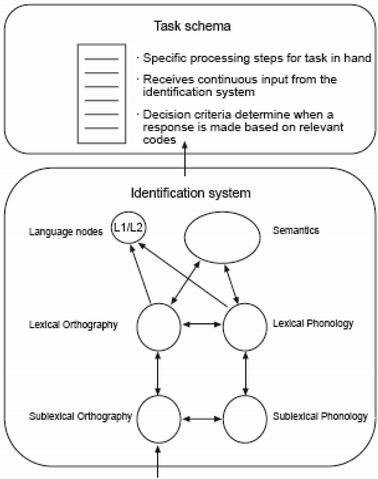
\includegraphics[scale=0.5]{Intro/Figures/biaplus.png}
\caption{The BIA+ model of word recognition \parencite[reprinted from][]{Dijkstra2002}}
\end{center}
\end{figure}

The word identification system deals with linguistic input to the model. The BIA+ posits an integrated lexicon (i.e., the words of each language are integrated into one “dictionary”) and shared semantics across the two languages. The word identification system is highly interactive. Upon “reading” a word, nodes for phonological and orthographic representations at the lexical and sublexical levels become active. Activation then spreads within and between the lexical and sublexical levels causing potential candidates to become more highly activated than other words. The higher levels of the model (i.e., the semantics level and language nodes) receive activation from the lower levels. In the semantic level, concepts receiving enough activation spread this activation back down to the lower levels further reinforcing the activation of potential lexical candidates. The language nodes are responsible for identification of the language being read. A crucial assumption made by the model is that the higher level nodes may only receive bottom-up activation. Furthermore, the language nodes may not send activation back down to the lower levels. Thus, prior knowledge of the intended language will not increase activation to nodes at lower levels. That is, the language nodes cannot function as a language filter. Instead, the nodes must be sufficiently activated through experience with a linguistic input.

While the word identification system handles linguistic input, the task schema deals with non-linguistic contexts. The task schema is responsible for accomplishing the task at hand (e.g., lexical decision, naming, etc.) and determining when a response should be made. In order to help with this decision, this level of the model receives constant input from the word identification system. A critical assumption of the BIA+ model is that the task schema (and, thus, non-linguistic context) does not infiltrate the word recognition system.  Evidence for this was shown by \textcite{Dijkstra2000} who demonstrated that the presence of stimuli and not expectations derived from instructions affected bilingual performance in an LDT.

% Dijkstra, de Bruijn, Schriefers, and ten Brinke (2000)

Given the assumptions of the BIA+ model it is easy to see how cross-language overlap will affect the recognition of words. Cognates, because of their close overlap in orthography, phonology, and meaning, will receive activation in both languages more quickly compared to words without similar overlap. Thus lexical decision or naming will be facilitated. On the other hand, when homographs are the input, the cross-language overlap with orthography and phonology may initially speed activation but the discrepancy in meaning will cause the system to have trouble identifying the language of the word thus slowing lexical decision or naming performance. Overall, the BIA+ predicts that a parallel access account with respect to language occurs in a bottom-up fashion. This parallel activity is not easily constrained by non-linguistic contexts. 

The question now is how linguistic contexts influence word recognition. Because the BIA+ model was designed to account for word recognition outside of sentence contexts, it makes no explicit predictions regarding linguistic contexts. However, as we shall see in the following section, there are specific linguistic contexts that may allow bilinguals to recognize words in a language-selective manner.

\section{In context word recognition}\label{Intro::InContext}
The previous studies reviewed thus far have been conducted asking participants to recognize single words. However, reading rarely involves the recognition of single words without any relation to one another. Instead, words are part of sentences which themselves are part of paragraphs. Likewise in speech, words are components of sentences in a discourse. Each level contributes a new layer of context. Because language use typically occurs in a rich context, out of context experiments provide an artificial environment for reading. For bilinguals, the ambiguity of language membership for each word may also be heightened. This may allow for parallel activation of both languages that would not otherwise exist in an environment with context. More recent research has sought to explore the role of sentence context on bilingual word recognition, investigating whether both language are still activated in parallel when a sentence is in one language alone. Only a handful of studies have examined this question, and the results have been interpreted in a variety of ways.

The fundamental question addressed by this most recent set of studies is whether evidence for nonselectivity can be seen in sentence context. Thus far, every study examining this question has come to the same conclusion: parallel activation does persist even when there is meaningful, unilingual context. This result is amazingly counterintuitive; an English word surrounded by other words that are unambiguously English activates words in another language.  It would seem that language nonselectivity is a fundamental property of the bilingual word recognition system and is does not arise as the result of experimental contexts. 

While the results of all studies converge on the fact that word recognition in sentence context is nonselective, there is disagreement on the issue of whether certain types of linguistic contexts can provide bilinguals a cue to the language of the sentence and work to lessen or even eliminate parallel activation of the unintended language. A set of studies has shown that semantic constraints can, at least sometimes, allow the system to function in a selective manner. The present study attempts to address this debate by examining another type of context that could work similarly to semantic constraints. 

%% The previous work reviewed thus far has been conducted asking participants to recognize single words.  However, reading rarely involves the recognition of single words without any relation to one another. Instead, words are part of sentences which themselves are part of paragraphs with each level contributing a new layer of context. Likewise in speech, words are components of sentences in a discourse. Language use typically occurs in a rich context. Out of context experiments may thus provide an artificial environment devoid of context, where the ambiguity of language membership of each word is heightened allowing parallel activation of both languages. More recent work has sought to explore the role of sentence context on bilingual word recognition, investigating whether both language are still activated in parallel when a sentence is in one language alone. Only a handful of studies have explored this question, and the results have been interpreted in a variety of ways. 

%Some researchers (e.g., Heridia at Psychonomics, and likely Duyck as well) would caution that the results of these in context studies are unclear, painting the picture for each study demonstrating nonselective access in context (e.g., Ducyk 2007, arguably Libben and Titone, Van Assche 2010, Van Assche 2009) there is a study that shows selective access (Schwartz and Kroll, Van Hell, arguably Libben and Titone, Chambers and Cook). However, if we are only allowed to decide that word recognition in sentence context is ``selective'' or ``nonselective'', then the results will appear mixed. If we instead allow language selection to occur on a continuum that ranges from nonselective to selective, then the results become clearer. Under this light, evidence from a variety of converging methodologies confirms that the bilingual word recognition system is, for the most part, nonselective in nature, though there are certain contexts (e.g., highly biased semantic constraints; Schwartz and Kroll, Chambers and Cooke, Libben and Titone) that allow the system to become selective. The selectivity seems to take place during later stages of processing (e.g., semantic integration). Importantly, forcing the system to become selective is not easy (e.g., Van Assche 2010). What has not yet been explored is whether there are other contexts that may allow the word recognition system to select a single language, and whether there exists a context that allows for selective access from the earliest stages in processing.  

\subsection{Evidence for nonselectivity in sentence context}\label{Intro::InContext::Evidence}
There is strong evidence that bilingual word recognition in sentence context is nonselective in nature. This is seen across a variety of methodologies, for example in word naming \parencite[e.g.,][]{Schwartz2006}; in lexical decision and translation \parencite[e.g.,][]{Baten2010, VanHell2008}; in eye-tracking measures of reading \parencite[e.g.,][]{Duyck2007, Libben2009, VanAssche2009, VanAssche2010}; and during auditory word recognition \parencite[][]{Chambers2009}. The unintended language is activated regardless of whether the less dominant L2 is in use \parencite[e.g.,][]{Baten2010,Chambers2009,Duyck2007, Libben2009, Schwartz2006,  VanAssche2010} or the more dominant L1 is use \parencite[e.g.,][]{VanAssche2009, Schwartz2006}. The degree of parallel activation is shown to be a function of the amount of cross-language overlap, suggesting parallel activation is not unique to cognates. Language nonselectivity seems to be a fundamental property of bilingual word recognition system. This finding is quite counterintuitive. It means that despite being aware that a sentence is entirely written in one language, a bilingual will activate both languages. The fact that a sentence has coherent semantics and syntax cannot eliminate activation of the unintended language. However, there is evidence that if a sentence is very strongly biased towards a single interpretation, parallel activity can be modulated.  

%%%% Methodology
Researchers have used a variety of methodologies to study language nonselectivity. Each method can provide a unique perspective on the phenomenon, particularly in what contexts and over what time-course it occurs. Importantly, research shows that regardless of the method used, bilingual word recognition is nonselective in nature. This cross-method comparison is important because it provides support that parallel activation is not task dependent. 

Initial evidence for parallel activation of two languages in sentence context came from behavioral tasks such as word-naming, lexical decision and translation \parencite[e.g.,][]{Baten2010,Schwartz2006, VanHell2008}. Parallel activation has also been demonstrated in auditory word recognition, suggesting that the phenomenon is not specific to written word recognition \parencite[][]{Chambers2009}. While the results of these tasks show the existence of parallel activation, they cannot speak to how early in processing the lexical candidates become activated. Are words in the two languages activated from the very beginning of processing, or do they only become activated during a later stage? The answer to this question comes from evidence from eye-tracking studies. They confirm that both languages are activated in parallel from the earliest stages of processing \parencite[e.g.,][]{Duyck2007, Libben2009, VanAssche2009,  VanAssche2010}. 

\textcite{Schwartz2006} were among the first to investigate bilingual word recognition in sentence context. They asked bilinguals to read sentences in both languages  across separate blocks. The sentences were presented word-by-word at a rapid pace, a method known as rapid serial visual presentation (RSVP). Target cognates and control words were marked in red and remained on the display until the participant spoke the name of the word. The time to begin speaking the word was recorded by a voice trigger. Schwartz and Kroll found that cognates were named faster than their matched controls in both the L1 and the L2. Cognate facilitation suggests that a sentence context is not enough to modulate language nonselectivity; bilinguals activated the lexical representations in both languages while reading in their native and second languages.

These results have also been corroborated by using a different set of behavioral tasks. \textcite{VanHell2008} asked bilinguals to make lexical decisions or to name the translations of target words (cognates or controls) that were embedded in sentences. Again, reaction times to translate or to perform a lexical decision were faster for cognates than for controls, suggesting that bilinguals activated both languages despite target words being embedded in a single language context. Evidence for cross-language activation during  lexical decision was corroborated by \textcite{Baten2010}. While parallel activation in a translation task may not be so surprising (the task demands that both languages are in use and likely to be activated by the participants) a lexical decision task does have this requirement.  Participants in an LDT are likely unaware that knowledge of a second language is important for the experiment. These replications suggest that the parallel activation as witnessed by \textcite{Schwartz2006} cannot be attributed to properties of the task or the materials. Instead, nonselectivity  seems to be a feature of the bilingual word recognition system. 

The finding of nonselectivity is not limited to the written word. \textcite{Chambers2009} show evidence for parallel activation during auditory word recognition. During auditory presentation of  sentences, French-English bilinguals viewed scenes containing 4 objects as their eyes were monitored, a methodology called the Visual World Paradigm (VWP). The visual displays included the target object mentioned in the sentence along with other objects that were unrelated to the sentence. Critical displays contained one object that was a homophone to the target object. For example, a participants might hear ``Marie va d\'{e}crire la \textbf{poule} / [Marie will describe the \textbf{chicken}]'' while viewing a scene that contained a chicken and a pool (the homophone). Chambers and Cooke found that participants were more likely to fixate on distractor homophones (e.g., pool) compared to unrelated objects, suggesting that they were activating English while listening to French sentences auditorily. 

Something that the behavioral studies and the VWP do not tell us is what the nature of the time-course of activation is. How early do participants begin considering options in both languages? If the word recognition system is truly nonselective, then parallel activation should occur immediately.  The use of eye-tracking while participants read sentences is well suited to address this question. 

Eye-tracking allows participants to read sentences naturalistically, as one might read a sentence in a newspaper. Participants are free to read at their own pace, and are able to regress back to earlier parts of the sentence in case something is misunderstood. While reading, the eye-movement patterns of the participants are monitored. The eye-movement record allows for a detailed analysis of the time-course of lexical activation. Early reading measures, such as first fixation duration, provide information about initial lexical access, while later reading measures provide information about semantic integration. 
\textcite{Duyck2007}, \textcite{Libben2009}, \textcite{VanAssche2009}, and \textcite{VanAssche2010} exploit this sensitivity of eye-tracking to show that words are activated in both languages in parallel from the earliest stages of recognition, and that coactivation remains indefinitely. In each of these studies, bilinguals read sentences that contained language-ambiguous words (cognates or homographs) and nonambiguous controls. The studies found that cognate words were fixated on for a shorter amount of time compared to control words while homographs were fixated on for a longer amount of time. Crucially, these effect were present from the earliest measures of reading (e.g., first fixation duration, which is taken to reflect initial lexical access) through later measures that reflect semantic integration. These eye-tracking studies show that during all points of word recognition, bilinguals have both languages activated in parallel.

The results of eye-tracking experiments investigating written and auditory word recognition converge with data from  behavioral studies to show that the finding of parallel activation is not dependent on the methodology being used. Next, we will see that, for the most part, the languages pairs that are used in these experiments and whether the languages are spoken as the L1 or L2 do not affect the overall result of nonselectivity in sentence context. 

%%%% L1-L2 and language pairs
An important consideration in assessing nonselectivity in sentence context is the direction of the coactivation. It is generally assumed that the L1 influences the L2 because the L2 is often the weaker language. However, evidence that the weaker  L2 can influence the stronger L1 provides a compelling case for the ubiquity of nonselectivity. A second consideration is whether the results can be replicated across a variety of language pairs, ensuring that nonselectivity is a feature of bilingual word recognition in general, not just recognition by a specific type of bilingual. Again, the number of in context studies is small, so more replication is necessary, but the preliminary set  suggests that the finding of nonselectivity is invariant to the languages spoken by the bilingual. 

The majority of evidence for nonselectivity in sentence context has been found for bilinguals reading in their L2. \textcite{Baten2010}, \textcite{Duyck2007}, \textcite{VanAssche2010},  \textcite{Libben2009}, and  \textcite{Schwartz2006} all tested bilinguals in English as their L2. \textcite{Chambers2009} recruited bilinguals that use French as their L2. All researchers find evidence for nonselectivity in sentence context. Because, it is often assumed that the L1 has an effect on the L2, parallel activation of the L1 while reading in the L2 may not be surprising. 

Yet, research has shown that bilinguals experience coactivation of the L2 even while reading in the stronger L1, though the number of studies is much more limited. In addition to presenting sentences in the L2, \textcite{Schwartz2006} also asked their participants to read sentences in a block of their L1 (Spanish). Likewise, \textcite{VanAssche2009} eye-tracked participants reading in their native language, Dutch. Both of these studies find cognate effects---evidence for language nonselectivity. These results provide striking evidence that even in L1 reading, a more practiced skill compared to L2 reading, bilinguals activate both languages in parallel. 

Considerably less research has systematically investigated the role of the specific languages in the degree of parallel activation within context. The languages pairs tested thus far have been Dutch and English \parencite[][]{Baten2010,Duyck2007, VanAssche2009, VanAssche2010}, Spanish and English \parencite[][]{Schwartz2006}, and French and English \parencite[][]{Chambers2009,Libben2009}. In the studies that have examined processing in the L2, the L2 has most often been English \parencite[][]{Baten2010,Duyck2007, Libben2009, VanAssche2010}, though Chambers and Cooke studied French as the L2. Because English and French are from different language families (Germanic and Romance) and because results of out of context studies have been replicated across a variety of different language pairs, concerns about confounds due to the language pairs should be ameliorated. Only, two studies have examined processing in the L1, one study investigates processing in Dutch \parencite[][]{VanAssche2009} and another in English \parencite{Schwartz2006}. Both Dutch and English are Germanic languages, which technically could confound the result because of language similarity. However, again results from out of context tasks suggest that the specific languages should not play a very large role; parallel activation should occur regardless of the languages.

A critique of the research supporting nonselectivity is that a majority of the evidence comes from cognates, which arguably have a special representation in the lexicon. Thus the argument can be made that evidence for parallel activation of two languages is really evidence for a special representation of cognates. If this is true, then it sheds doubt on the usefulness of the cognate effect as a measure of cross-language parallel activation. The cognate effect may result from a special representation. This potential confound can be addressed by investigating the role of cross-language overlap in word recognition. If the cognate effect is driven by special representation, then word recognition times should not differ as a function of the degree of overlap because all cognates are special. In contrast, if the cognate effect is really a marker of parallel activation, then we should see graded effects that are dependent on the amount of cross-language overlap.  

A subset of the studies discussed above show evidence that the size of the cognate effect  depends on the degree of cross-language overlap. Cross-language overlap can be operationalized in terms of orthographic overlap and phonological overlap. For example, \textit{hotel} and \textit{ship} are both cognates with Dutch. \textit{Hotel}, however, has complete orthographic overlap with Dutch whereas \textit{ship} is written as \textit{schip} in Dutch, containing a slight difference in orthography. Similarly, words that are written the same across languages often differ in their pronunciation (phonological overlap) or in their meaning (i.e., homographs). The typical finding has been that words with less cross-language overlap tend to elicit slower reaction times while words with greater overlap are recognized faster. This justifies the use cognate effect as a marker of parallel activation. 

\textcite{Duyck2007} conducted a discrete analysis using their eye-tracking data  to show that cross-language overlap affects the presence of the cognate effect. In their materials, they included cognates and noncognate words, and the cognate items were further split into identical cognates (e.g., hotel) and nonidentical cognates (e.g., \textit{ship}-\textit{schip}). Duyck et al. found that identical cognates were fixated on for a shorter amount of time compared to matched noncognate control words. However, this difference was not significant for nonidentical cognates. This finding provides preliminary evidence for the idea that not all cognates are processed equally. Cognates with complete orthographic overlap elicit a greater cognate effect, while the nonidentical cognates elicit a smaller effect. This small effect was apparently not detectable by Duyck et al.'s analysis.  

%An alternative explanation for this lack of cognate effect for nonidentical cognates exists. The sentences in this experiment may have been providing lexical restrictions, albeit weak ones, to language of the sentence. The effect of these restrictions in negating parallel activity only emerged when parallel activation was weaker because of incomplete orthographic overlap. This alternate explanation is complementary to the hypothesis that incomplete orthographic overlap alone is the determinant of the lack of cognate effect. However, it is important to disentangle the role, if any, that the sentence context plays from the role that orthographic overlap plays in parallel activation of two languages. 

%Duyck et al. (2007) conducted two control studies (out of context lexical decision and in context lexical decision) to provide support the idea that the lack of a cognate effect for nonidentical cognates is due to orthographic overlap  and not to sentential context. They showed that LDT reaction times to cognate words (in and out of context) were influenced by the degree of orthographic overlap: a decrease in orthographic overlap resulted in greater reaction times. This correlation also held for reading times in the eye-tracking experiment. Yet, in both LDTs there was still a significant cognate effect for the nonidentical cognates where there was none in the eye-tracking experiment. The presence of a cognate effect for nonidentical cognates sentential LDT suggests that the nonidentical cognates, though they lacked complete orthographic overlap, were sufficiently able to elicit parallel activation of both languages in the context of a sentence. 

%The presence of parallel activation for nonidentical cognates in the sentential lexical decision task leaves open the possibility that the eye-movement record was unable to detect weak parallel activation despite the common assumption that eye-tracking is a more sensitive measure than behavioral tasks. This could occur, counterintuitively, because the method is very sensitive, providing very fast reaction times (on the order of 200ms in Duyck et al., 2007) in comparison to LDT reaction times (around 700ms) for example. Such small effects may be difficult to detect with very fast reaction times and instead may require a measure that magnifies the differences, something to be kept in mind when designing a study that might result in small effects. Overall, the results of the series of studies conducted by Duyck et al. suggest that a sentence context alone is not sufficient to override parallel activation of the L1 when reading in the L2.

%The authors show that the degree of parallel activation is a function of cross-language overlap. Cognates that have greater orthographic overlap across languages tend to be read faster. Duyck et al. conduct a  discrete analysis by comparing nonidentical cognates to identical cognates and show that only identical cognates provide evidence for parallel activation. This finding is honed by Van Assche et al. who conduct a regression analysis to show that this effect is actually continuous: the cognate effect decreases continually as a function of orthographic overlap.

While the results of \textcite{Duyck2007} suggest that orthographic overlap influences the time to identify a word, a discrete difference between identical and nonidentical cognates does not defeat the theory that cognates have a special representation. One could argue that while identical cognates are specially represented, nonidentical cognates are not cognates are not, explaining why \textcite{Duyck2007}  not see facilitation for nonidentical cognates. A more fine grained analysis can adjudicate whether cognates are somehow special.

\textcite{VanAssche2009} and \textcite{VanAssche2010} found continuous effects of cross-lingual overlap on reading times in the L1 and in the L2. Where \textcite{Duyck2007} categorized cognates into discrete groups (identical and nonidentical), \textcite{VanAssche2009} calculated the orthographic overlap of each target word and its translation according to the method by \textcite{VanOrden1987}. This method provides a numerical measure of overlap between two words by taking into account such factors as number of letters, number of paired adjacent letters, whether the words share the same first or last letter, etc. This measure of overlap was then entered as a predictor into linear mixed-effects regression models for each of the eye-tracking measures of interest (first fixation duration, gaze-duration, and regression-path duration). While overall model fits were not included in the results, the authors found a significant effect of orthographic overlap on reading times. The time to read a word was inversely proportional to the degree of overlap; as overlap decreased reading times increased. This shows that readers utilized this  lexical information during word recognition. 

\textcite{VanAssche2010} further show that the degree of phonological overlap influences bilingual word recognition and can be used as another continuous  measure of cognate status. They measured the degree of phonological overlap  by asking a group of participants, independent from their main experiments, to rate how similarly a word and its translation sounded. These ratings were aggregated to determine degree of overlap. When phonological similarity was entered into the regression model, the authors found an inversely proportional relation to reaction times, similar to that of orthographic overlap.

The results of \textcite{Duyck2007}, \textcite{VanAssche2009}, and \textcite{VanAssche2010} illustrate that the degree of cross-lingual overlap  influences how bilinguals recognize words in sentence context and that this effect is continuous. As words across two language increase in the degree of overlap, the speed at which they are recognized increases. This finding is important because it shows that cognate status per se is not what influences recognition. Recognition is influenced by the degree of overlap between a word and its translation equivalent. Therefore it is correct to assume that the cognate effect is a measure of parallel activation of the bilingual's two languages not as proof of a special representation of cognates.

Taken together, the results of the in context studies presented here all show that language nonselectivity cannot be overcome by a sentence context alone. Words become activated in both languages according to their degree of overlap across languages despite the coherence created by the semantics, syntax, and language of a sentence. The parallel activation is so pervasive that it persists while bilinguals read sentences in their stronger native language, not only during L2 reading.  

Yet it would seem that at some point, a bilingual should be able to ``choose'' a language. After all, bilinguals can successfully make lexical decisions in a sentence context, nor do they have a problem assembling the meaning of a sentence. Given the pervasiveness of nonselectivity in sentence context, a second goal of in context word recognition research has been to explore whether there are any linguistic factors that might allow bilinguals to make a language selection.

\subsection{The role of semantic constraints}\label{Intro::InContext::SemanticConstraints}
While all studies converge on the finding that word recognition is nonselective within a sentence context, they diverge on whether recognition may become selective under certain conditions, namely following a highly constrained semantic context. A subset of the studies examined above illustrates that patterns of word recognition following a highly biased context are consistent with the predictions made by a language-selective access account. In highly constrained  contexts, cognate facilitation is eliminated \parencite[the \textit{semantic constraint effect}; e.g.,][]{Chambers2009,Libben2009, Schwartz2006, VanHell2008}. However, there is disagreement in the literature as to whether the locus of the effect actually stems from language-selectivity, or whether it is the result of another factor, such as a confounding of the methods or a floor effect caused by the speeded processing due to semantic constraints. Furthermore, one study has failed to find the semantic constraint effect \parencite[e.g.,][]{VanAssche2010}. Despite the criticisms of semantic constraints, the effect seems to be reliable. Yet, semantic constraints cannot be the only way that a bilingual comes to choose a language. After all, not every sentence is highly semantically constrained. Other factors that provide language-specific cues, such as the syntax, may induce language-selective access.   

The semantic constraint effect has been replicated with a variety of methods including lexical decision and translation \parencite[][]{VanHell2008}, eye-tracking during reading, and with the Visual World Paradigm \parencite[][]{Chambers2009,Libben2009}. The eye-tracking record shows that when semantic constraints have an effect, it occurs during later stages in processing \parencite[][]{Libben2009}. Because the effect of semantic constraints can be seen with a variety of methods, from behavioral to eye-tracking, the effect is likely not due to the methodology. However, the debate about whether speeded processing creates a floor effect is still open. The current study will approach the question of whether word recognition can become selective by investigating whether another sentential factor, language-specific syntactic constraints, can eliminate or reduce parallel activation. 

\textcite{Schwartz2006} demonstrate that a sentence which is highly constrained in its interpretation appears to eliminate the cognate effect. Schwartz and Kroll varied the semantic constraint of their sentences such that half of the sentences contained a highly predictable semantic contexts (i.e., \textit{high constraint}) while the other half did not (i.e., \textit{low constraint}). Constraintedness was determined by an offline sentence completion task. The target word of each sentence was removed along with any material following the target. A set of participants who did not complete the main experiment  asked to complete each sentence. If the participants were highly likely to complete a sentence with the actual target word, the sentence was rated as high constraint. If a variety of words followed a sentence, it was rated as low constraint. 

\textcite{Schwartz2006} found cognate facilitation only in the low constraint sentences. In sentences with a high semantic constraint, the authors found that all target words were named faster. This signifies that the biased context helped participants to access the upcoming target word. Importantly, the authors failed to find a cognate effect for target words following a high semantic constraint.  The cognate facilitation effect in low constraint sentences signifies that a sentence context alone is not enough to constrain word recognition to one language. However, additional semantic cues may provide lexical restrictions to language, resulting in a modulation the cognate effect. 

The finding of apparent selective access in high constraint sentences has been criticized on two grounds. First,  the elimination of the cognate effect may be the result of the method that Schwartz and Kroll used to investigate word recognition (i.e., word naming). Second, the elimination of the cognate effect in high constraint sentences may be the result of the facilitation that occurs following a biased semantic context. That is, because high constraint sentences speed lexical access, word recognition in these sentences may reach a floor and  cognate facilitation may no longer be witnessed. Each critique warrants further explorations, and with the use of converging methodologies, they can begin to be addressed. 

%%%% Methods
The semantic constraint effect cannot be due to the methods used by \textcite{Schwartz2006}. The effect has been replicated using other behavioral methods as well as with eye-tracking methods \parencite[e.g.,][]{Chambers2009,Libben2009,VanHell2008}. The eye-tracking record during reading suggests that the effect of semantic constraints occurs during later stages of word recognition, meaning that word recognition is initially nonselective. While converging methods confirm that semantic constraints eliminate the cognate effect, they cannot confirm that this modulation is due to language-selective access. The reduction in the cognate effect may be due to speeded access of semantic constraints creating a floor effect that over-shadows an effect of cross-language overlap. 

\textcite{VanHell2008} show that semantic constraints modulate the cognate effect during word recognition while bilinguals read sentences and were asked to make either a lexical decision or to translate the target words. When targets followed a high semantic constraint (which again facilitated reaction times to identify targets), the difference between cognates and controls was reduced, and in lexical decision the difference was eliminated. A similar finding occurred during auditory word recognition. \textcite{Chambers2009} found  that following sentences containing a high semantic constraint, fixations toward homograph distractor pictures were greatly decreased when compared to fixations in low constraint sentences. 

Following highly semantically constrained sentences, the degree to which both languages were activated was greatly decreased in line with the findings of Schwartz and Kroll. Because the constraint effect was replicated with a different set of behavioral methods, it signifies that the findings of Schwartz and Kroll did not depend on the word naming method they used. 

%Like Schwartz and Kroll (2006), Van hell and de Groot included sentences that had a high semantic constraint in their materials. Recall that they asked one group of participants to make  a lexical decision on the target words while translated the targets and that translation and lexical decisions were faster for cognates when the sentences were low semantic constraint. Crucially, w

Behavioral tasks, such as lexical decision, translation, and word naming, rely on the response made by a participant to a stimulus. Responses  tell us about the later stages of word recognition---the end result of the process. Information about the  earliest stages of the process is potentially lost. Thus, it is conceivable that in high constraint sentences, word recognition  proceeds in an initially nonselective manner and then becomes selective downstream. If this theory were true, behavioral methods such as those used by \textcite{Schwartz2006} and \textcite{VanHell2008} might fail to capture evidence for this initial nonselectivity. While the Visual World Paradigm used by \textcite{Chambers2009} provides a good temporal measure of the word candidates participants are considering, the analysis they conducted was not fine-grained enough discern whether the semantic constraint effect began initially or later on. Analyses of fixations during sentence reading are sensitive enough to adjudicate between early and late processing differences.  
 
\textcite{Libben2009} provide striking data that suggest word recognition in high constraint sentences proceeds in an initially nonselective manner but becomes selective over time as the meaning of the sentence is integrated. They show that in high constraint sentences cross-language facilitation and inhibition were only present in early measures of reading (e.g., first-fixation duration). Later measures (e.g., regression path) showed no significant differences between language-ambiguous stimuli and control words. This result highlights the fact that the word recognition system is profoundly nonselective at early stages of processing, but that semantic constraints can allow the system to become selective over time. It also further shows that the semantic constraint effect is not unique to behavioral methods, such as word naming. 

Findings from a variety of methods provide evidence that semantic constraints can eliminate activation from the unintended language. This finding is not method-specific, though there are differences in how methods illustrate details about the time-course of processing. While the semantic constraint effect is not due to the methodology used,  locus of the effect is still in question; the elimination of the cognate effect may be due to the fact that semantic biases increase word recognition speed. This speed increase may create a floor effect that diminishes the detectability of the cross-language activity. 

%%%% Speed of semantic constraints
Semantic constraints reliably increase the rate at which upcoming words are recognized, and we have seen that semantic constraints decrease or eliminate effects that are known to measure parallel activation (e.g., cognate effect and homograph inhibition). However, the locus of this modulation is in question. It could stem from two possible sources: language-selective access cause by increased lexical cues due to the constraint, or, more trivially, a loss of analytical power due to the decrease in reaction times due to the semantic constraint. Much of the prior research cannot address this question, except for, possibly, the results of Van Hell and De Groot.  

The idea behind the floor effect theory is that participants become so fast at predicting an upcoming word, the cognate effect can no longer be measured. Cross-language activation is still present, however the effect size is so small it cannot be measured. This theory can be tested by examining a situation in which there is a semantic constraint but no floor effect. In such a situation, the theory would predict that a cognate effect would be present, and the magnitude of the effect should be no different than in a low constraint sentence. A difference in the sizes of the cognate  effects would indicate that the semantic constraint is in some way affecting the degree of parallel activation.

The translation task of \textcite{VanHell2008} provides the situation outlined above. In their experiments, participants translated target words that were embedded in high and low constraint sentences. Translation is a more difficult task for participants compared to lexical decision or word naming. Hence, reaction times are slower (though no statistical analyses were conducted to test this). Because reaction times were no longer at floor, role of semantic constraints can be investigated. Van Hell and De Groot found cognate effects in both high and low constraint sentences during translation. However, counter to the predictions made by the floor effect theory, the cognate effect was smaller in the high constraint condition, indicating that although participants coactivated both languages during the translation, this coactivation was less when the context was biased towards a single interpretation. This modulation is likely due to a decrease in parallel activation and not a floor effect because reaction times in the task were slower overall. 

%%%% Failure to find semantic constraints
Not all studies have managed to find evidence for the semantic constraint modulation of the cognate effect. Though, failure to find an effect is not evidence that no effect exists, especially in the presence of other positive evidence. It may be that semantic constraints do not always allow for words to be selectively accessed from the lexicon. 

\textcite{VanAssche2010} failed to find evidence that semantic constraints modulate the cognate effect, despite the inclusion of  sentences that were rated as being very high constraint compared to previous studies. Instead, their Dutch-English bilinguals read cognate words significantly faster than noncognate words in both low and high constraint sentences; the magnitude did not change. According to Van Assche et al. ``this contrasts with Libben and Titone (2009) who found cognate facilitation only in early comprehension measures... Instead, our results suggest that the influence of such factors on the language-selectivity of lexical access is rather limited...'' This result also contrasts with Schwartz and Kroll, Van Hell and De Groot, and Chambers and Cooke. As we know from statistics, lack of a significant effect is not evidence that there is no effect. Instead there are likely many factors which the authors did not consider that likely result in the lack of the effect.  

The main reason that \textcite{VanAssche2010} failed to find an effect was likely due to the sizes of their cognate effects. For some of the measures, the effects were less than 10ms. These effects are so small that the number of participants they recruited is much higher than in previous studies (e.g., 60 participants). A sub-10 ms effect, in  addition to potentially not being a meaningful difference, leaves less room to find a detectable interaction when the effect is expected to decrease.

In this study, the more proficient language and dominant language (i.e., Dutch) of the environment was inactive, so cognate effects should have been rather large \parencite[e.g.,][]{Jared2001, Marian2003, VanHell2002}. Why were the effects so small?  \textcite{VanAssche2010} chose to use exclusively nonidentical cognates as a tool to measure of parallel activation. As we saw earlier, nonidentical cognates tend to elicit less parallel activation (and perhaps none at all) because of their lack in cross-language overlap. Furthermore, in \textcite{Duyck2007} the group failed to find any cognate effects on nonidentical cognates as a group. In this light, it is not surprising that Van Assche et al. struggled to find a cognate effect and failed to finsd evidence for an interaction. 

While failure to find the semantic constraint modulation does not prove that the effect does not exist, the findings of \textcite{VanAssche2010} do suggest that decreasing parallel activation is not always as easy as including a high semantic constraint. Furthermore, not every sentence contains a semantic constraint, thus there may be several other factors that allow bilinguals to come to a language decision. 

\section{The present investigation}\label{Intro::PresentInvestigation}
Most researchers assume that the semantics is shared across language. Therefore there is no reason a priori that the meaning of a sentence should provide strong language cues. On the other hand, it is well known that syntax differs across languages. If any linguistic construct should provide language cues, then it should be the syntax. The goal of the  present investigation  is to  explore whether language-specific syntactic constraints allow for language-selective access. While nobody has examined this question, there is evidence from an out of context task and an in context task that hints that aspects of the syntax may be important during word recognition.

\textcite{Sunderman2006} showed that grammatical class differences (a morphosyntactic property) can reduce lexical form interference from the other language. Relatively proficient English-Spanish speakers made translation recognition judgments about word pairs in Spanish and English (i.e., ``Are these two words translations of one another?''). Critical word pairs required a ``no'' response, and a subset of critical items were related in lexical form (e.g., \textit{mano}-\textit{man}). When the two words belonged to the same grammatical class (e.g., noun-noun),  Sunderman and Kroll found lexical interference compared to control items (e.g., \textit{casa}-\textit{man}). However, when the two words differed in their grammatical classes (e.g., noun-verb), the lexical interference was dramatically reduced, suggesting that the degree of lexical interference depended on grammatical class overlap. 

A similar result was found by \textcite{Baten2010} for bilingual participants reading in sentence context. Participants performed an English lexical decision for target words embedded in sentences. Homographs elicited a facilitation effect when the homograph and its translation shared grammatical class, suggesting that both languages were activated. However, when the grammatical class differed across the two languages the facilitation effect was eliminated, consistent with language-selective access. The results of \textcite{Sunderman2006} and \textcite{Baten2010}  hint that syntax may play a role in modulating  influence from the unintended language.

The present investigation explores the role of syntax in allowing for language-selective activation by asking Spanish-English bilinguals to read sentences that are language-specific to Spanish in their syntax. We operationalize Spanish-specific syntactic constraints as the inclusion of proclitics and the dropping of the subject of an object relative clause before the target word of the sentence is reached. Spanish-specific syntax is exemplified in \ref{lasmonjas2} (target word: \textit{directora}, a cognate).

\ex.\label{lasmonjas2} Las monjas \textbf{le} llevaron las mantas que \textbf{[pro]} hab\'{i}an bordado a la directora del orfanato.\\
      The nuns \textbf{[ ]} took the quilts that \textbf{they} had embroidered to the director of the orphanage.

If the presence of Spanish-specific syntactic constructions in a sentence allow the reader or listener \textit{zoom in} to the target
language \parencite[e.g.,][]{Elston-Guttler2005}, then word recognition should proceed in a language-selective selective manner. That is, cognates
embedded in sentences with language-specific syntax (and with a low
semantic bias) should be accessed as if they are a word only in the
language of that sentence (i.e., a noncognate word). However, following language-general syntax, word recognition should proceed in a nonselective manner, in line with previous studies. Monolingual control experiments will confirm that any cognate or syntactic specificity effects are due to the experimental manipulations and not to idiosyncratic properties of the stimuli.

The experiments in the current investigation are laid out as follows. Experiment 1 implements a word naming task to replicate the cognate facilitation effect outside of sentence context. Experiment 2 uses the Rapid Serial Visual Presentation task to present cognate and noncognate control words in sentence contexts that contain language-general (low syntactic constraint) and language-specific syntactic constraints (high syntactic constraint). A block of Spanish sentences will contain both low and high syntactic constraints while a block of English sentences contain only low syntactic constraints. Experiments 3 and 4 are English and Spanish monolingual control experiments.  

